\documentclass{ti2}

% Dateikodierung ist utf8
\usepackage[utf8]{inputenc}
\usepackage{listings}
\usepackage{ucs}
\usepackage{color}
\usepackage[dvipsnames]{xcolor}
\usepackage{hyperref}
\usepackage{fancyvrb}
\usepackage{wrapfig,lipsum,booktabs}
\usepackage{adjustbox}
\usepackage{lmodern}
\usepackage{enumitem}
\setlist[enumerate,1]{start=0} % only outer nesting level
% redefine \VerbatimInput
\RecustomVerbatimCommand{\VerbatimInput}{VerbatimInput}%
{fontsize=\footnotesize,
 %
 frame=lines,  % top and bottom rule only
 framesep=2em, % separation between frame and text
 rulecolor=\color{Gray},
 %
 label=\fbox{\color{Black}test.txt},
 labelposition=topline,
 %
 commandchars=\|\(\), % escape character and argument delimiters for
                      % commands within the verbatim
 commentchar=*        % comment character
}
\lstset{ 
language=C++,                % choose the language of the code
basicstyle=\footnotesize,       % the size of the fonts that are used for the code
numbers=left,                   % where to put the line-numbers
numberstyle=\footnotesize,      % the size of the fonts that are used for the line-numbers
stepnumber=1,                   % the step between two line-numbers. If it is 1 each line will be numbered
numbersep=5pt,                  % how far the line-numbers are from the code
backgroundcolor=\color{white},  % choose the background color. You must add \usepackage{color}
showspaces=false,               % show spaces adding particular underscores
showstringspaces=false,         % underline spaces within strings
showtabs=false,                 % show tabs within strings adding particular underscores
frame=single,           % adds a frame around the code
tabsize=2,          % sets default tabsize to 2 spaces
captionpos=b,           % sets the caption-position to bottom
breaklines=true,        % sets automatic line breaking
breakatwhitespace=false,    % sets if automatic breaks should only happen at whitespace
escapeinside={\%*}{*)},          % if you want to add a comment within your code
inputencoding = latin1,
literate={ö}{{\"o}}1
           {ä}{{\"a}}1
           {ü}{{\"u}}1
}

\usepackage{xcolor}
  \definecolor{sx-yellow}{RGB}{249,245,233}
  \definecolor{sx-orange}{RGB}{224,215,188}
\usepackage[most]{tcolorbox}

\makeatletter
\renewenvironment{quote}{%
  \vskip 10\p@
  \parindent\z@
  \tcolorbox[
    breakable, sharp corners,
    boxrule=\z@, boxsep=\z@,
    left=\z@, right=\z@,
    top=\z@, bottom=\z@,
    colback=sx-yellow
  ]
  {\color{sx-orange}\d@ublerule}
  \vskip 5\p@
  \list{}{\rightmargin\leftmargin}%
  \item\relax
}{%
  \endlist
  {\color{sx-orange}\d@ublerule}
  \endtcolorbox
  \vskip 5\p@
}
\def\d@ublerule{\hrule\@width\hsize\kern 1.5\p@\hrule\@width\hsize}
\makeatother

\setlength{\parindent}{0pt}
\begin{document}

% Nr, Abgabedatum, Gruppenleiter, Gruppenname, Name1...Name4
\Abgabeblatt{4}{28.11.2016}{Marc/Bingbin}{C02}%
                {Rene Engel}{Dennis Jacob}%
                {Jan Schoneberg}%
                


\section*{Aufgabe 1}
\subsection*{Implementierung}
\lstinputlisting{Loesung/04/ti2sh.cc}
Für die Lösung der Aufgabe 1 wurden zuerst mehrere Hilfsfunktionen definiert. \textit{is\_in\_dir} stellte fest, ob ein gegebener Name als Datei oder Ordner in dem gegebenen Pfad vorhanden ist. Dies vereinfacht das durchsuchen der in der \textbf{PATH}-Variable gegebenen Pfade. Die Methode \textit{dirExists} prüft, ob der gegebene Pfad existiert und ein Ordner ist. Dies vereinfacht das Behandeln von Pfadwechseln. Die Methode \textit{split\_str} liefert eine Liste von \textit{std::string}s zurück, die durch das Trennen des gegebenen Strings am \textit{Regex} entsteht. \textit{signalHandler} ist ein Callback für eingehende Signale.

In der \textit{main}-Methode wird zuerst das nächste Kommando geholt und danach geprüft, ob es eine Anweisung für die Shell direkt ist. Eine solche Anweisung könnte \textit{exit} oder \textit{cd <dir>} sein. Bei einem \textit{exit} wird die Shell beendet. Die Anweisung cd benötigt eine etwas aufwendigere Behandlung. Zuerst wird geprüft, ob das gegebene Argument ein existierender Ordner ist. Ist dies der Fall, wechselt die Shell zu dem Ordner und gibt den jetzt aktuellen Pfad aus. Wird kein Argument gegeben, so holt sich die Shell die Umgebungsvariable für den \textit{home}-Ordner, prüft ob er existiert und wechselt zu diesem. Ist keine solche Variable gegeben oder Fehlerhaft, wird eine entsprechende Fehlermeldung ausgegeben. Sollte der Parameter ein nicht existierender Ordner sein, wird auch dies ausgegeben. Danach wird einmal der übergebene Befehl mit der Information, ob dieser im Hintergrund ausgeführt wird, ausgegeben und eine Variable entsprechend gesetzt. Als nächstes wird geprüft, ob die, in der Umgebungsvariable \textbf{PATH} definierten Pfade, das entsprechende Programm für das eingegebene Kommando beinhalten. Dafür wird zuerst die Variable \textit{bin} temporär auf den Pfad \textit{/usr/bin/} gesetzt. Die Umgebungsvariable wird dann in \textit{env\_path} zwischen gespeichert und danach mit \textit{split\_str} aufgeteilt. Dann iteriert eine Schleife über jeden Eintrag in der Pathvariable und sucht den Befehl. Wird der Befehl gefunden, so wird die Variable \textit{command\_found} auf \textit{true} gesetzt und die Schleife beendet.
Existiert das Programm nicht, so wird eine Fehlermeldung ausgegeben. Danach wird aus dem Pfad und dem Namen des Programms ein \textit{char}-String erzeugt. Jetzt wird die Callback-Methode \textit{signalHandler} für das Signal \textit{SIGCHLD} registriert. Mit dem Systemaufruf \textit{fork} wird ein neuer Kindprozess erzeugt. Sollte dies nicht funktioniert haben, so wird eine Fehlermeldung ausgegebenen. War der \textit{fork}-Aufruf erfolgreich, wird der Befehl mit den restlichen Parametern ausgeführt. Wird der Kindprozess im Vordergrund ausgeführt, so wartet der Elternprozess auf dessen Beendigung. Der Signalhandler wird nicht aktiv (durch entsprechende if Bedingung) das das Kind bereits in Elternprozess \glqq eingesammelt\grqq wurde.  Wird der Kindprozess im Hintergrund ausgeführt wird nach dessen Terminierung das Signal \textit{SIGCHLD} durch den Signalhandler bearbeitet und der Kindprozess \textit{eingesammelt}
\newpage
\subsection*{Test}
Der Test der TI2 Shell erfolgte im wesentlichen manuell. Dazu wurden in der Shell (Testrechner x02) verschiedene Befehle (u.a. cd, exit, ls, echo) eingeben und die Ausgaben beobachtet. Diese waren wie erwartet, z.B. bei \textit{echo Test} die Ausgabe \textit{Test}. Da die Einleseroutine vorgegeben war, haben wir diese nicht in unsere Tests einbezogen. Außerdem muss die Ein-/Ausgabeumlenkung nicht getestet werden. Es bleibt also nur noch folgendes zu testen: \\
\textbf{1.} Fehlerfälle \\
\textbf{2.} starten der Prozesse im Hintergrund \\
\textbf{zu 1.}\\
Der Test erfolgte ebenso hauptsächlich manuell. Es wird im Fehlerfall jeweils eine entsprechende Fehlermeldung ausgegeben. Folgende Fehlerfälle haben wir identifiziert und geprüft ob entsprechende Fehlermeldungen ausgegeben werden: \\
ungültige Befehlen(z.b. unvollständige Befehle oder der Aufruf von Programmen, die nicht in PATH liegen), die Fehlermeldung \glqq Command not found \grqq  \\
cd ohne weiteren Parameter, wenn kein gültiger Pfad in \textit{HOME} liegt, die Meldung \glqq Home does not exist! \grqq  \\
cd mit ungültigem Pfad, die Meldung \glqq Directory does not exist! \grqq \\
\textbf{zu 2.} \\
Um zu prüfen ob ein Prozess im Hintergrund gestartet wird haben wir ein kleines Skript geschrieben. Dort wird ein Prozess benötigt, der auf die Konsole schreibt. Da der \textit{Echo} Befehl auf den x-Rechnern in \textit{/bin} liegt und dieses Verzeichnis (zumindest auf dem x02 Rechner) nicht in \textit{PATH} war haben wird dieses Verzeichnis zunächst \textit{PATH} hinzugefügt. Auch das Verzeichniss \textit{/usr/bin} wird \textit{PATH} hinzugefügt, falls dies noch nicht geschehen ist. Auch dort liegen einige Programme und auf einigen Unix ähnlichen Betriebssystemen, wie openSuse, sogar die meisten Programme. 
\lstinputlisting[captionpos=b,firstline=1, firstnumber = 1,lastline=34]{Loesung/04/Test.sh}
Danach beginnen die eigentlichen Testfälle. 
\lstinputlisting[captionpos=b,firstline=35, firstnumber = 35]{Loesung/04/Test.sh}
Zunächst wird die TI2 Shell so aufgerufen, dass der Befehl \textit{echo} im Hintergrund läuft und dann die Befehle \textit{sleep} und nochmal \textit{echo}. Da der erste \textit{echo} Befehl im Hintergrund aufgerufen wurde und danach ohne Verzögerung sleep ausgeführt wird, erscheint die Ausgabe vom ersten \textit{echo} erst nach beiden! \textit{comand...} Ausgaben in Zeile 3. \\ \\
Im nächsten Testfall wird der erste \textit{echo} Befehl im Vordergrund gestartet und erst nachdem dieser die Ausgabe getätigt hat, wird mit sleep weiter gemacht. Deshalb befindet sich die Ausgabe in Zeile 2. \\ 
Dieses wird im Testskript automatisch ausgewertet und sowohl formatiert als auch mit sinnvollen Meldungen in die Datei \textit{TestResults.txt} geschrieben. 
\lstinputlisting[captionpos=b,firstline=1, firstnumber = 1]{Loesung/04/TestResults.txt}
Der letzte Testfall prüft zusätzlich zu den manuellen Tests eine Fehlerhafte Eingabe. Die TI2 Shell führt keinen Befehl aus, sondern es erscheint die Ausgabe \glqq Command not Found\grqq .
\section*{Aufgabe 2} 
%Umrechnung Byte KiB gleich
Bei der folgenden Aufgabe wird stets in KiB gerechnet, da die Rechnung in Byte äquivalent aber umständlicher ist. Lediglich der k Wert ist anders, was folgende Beispielrechnung belegt. 
\begin{center}
$10 KiB = 10240 Byte$\\
$log_2(10240) \approx 13,3 $\\
$2^{14} Byte = 16384 Byte = 16 KiB = 2^4 KiB$\\
\end{center} 
Weiterhin werden die Anforderungen mit Buchstaben eindeutig nach folgender Tabelle durchnummeriert.
\begin{table}[htbp]
\begin{adjustbox}{max width=\textwidth}
\begin{tabular}{|l|l|l|}
\hline
Anforderung & Speicher (KiB) & Block (KiB) \\ \hline
A  & 10 & 16 \\ \hline
B & 12 & 16 \\ \hline
C & 3 & 4 \\ \hline
D & 16 & 16 \\ \hline
E & 1 & 4 \\ \hline
F & 20 & 32 \\ \hline
G & 2 & 4 \\ \hline
\end{tabular}
\end{adjustbox}
\end{table}
\\In den Speicherblöcken stehen sowohl der Buchstabe der Anforderung als auch die Blockgröße in KiB. Ein kleines f bedeutet, dass der Block frei ist. Über den Speicherblöcken steht die Startadresse der jeweiligen Blöcken. 
\subsection*{Aufgabe 2a)}
Im folgenden ist der Speicher für die ersten Anforderungen dargestellt. \\
\begin{table}[htbp]
\begin{adjustbox}{max width=\textwidth}
\begin{tabular}{|l|l|l|l|l|}
\hline
Anforderung & 0 & 16 & 32 & 48 \\ \hline
A  & \multicolumn{ 4}{l|}{f64} \\ \hline
 & \multicolumn{ 2}{l|}{f32} & \multicolumn{ 2}{l|}{f32} \\ \hline
 & f16 & f16 & \multicolumn{ 2}{l|}{f32} \\ \hline
 & A16 & f16 & \multicolumn{ 2}{l|}{f32} \\ \hline
B & A16 & B16 & \multicolumn{ 2}{l|}{f32} \\ \hline
C & A16 & B16 & f16 & f16\\ \hline
\end{tabular}
\end{adjustbox}
\end{table}
\\Im folgenden ändert sich der Speicherbereich von Adresse 0 bis 31 nicht mehr, da dieser vollständig gefüllt ist und kein Block wieder frei gegeben wird. Deshalb wird der restliche Bereich (32 bis 63) näher betrachtet. 
\begin{table}[htbp]
\begin{adjustbox}{max width=\textwidth}
\begin{tabular}{|l|l|l|l|l|}
\hline
Anforderung & 32 & 36 & 40 & 48 \\ \hline
C & \multicolumn{3}{l|}{f16} &f16  \\ \hline
 & \multicolumn{ 2}{l|}{f8} &f8& f16 \\ \hline
 & f4 & f4 &f8 & f16 \\ \hline
 & C4 & f4 & f8 & f16 \\ \hline
D & C4 & f4 & f8 & D16 \\ \hline
E & C4 & E4 & f8 & D16 \\ \hline
\end{tabular}
\end{adjustbox}
\end{table}
\\Da es keinen ausreichend großen freien Block gibt, um die Anforderung F zu erfüllen, muss mehr Speicher von Betriebssystem geholt werden (brk() System Call). Der zusätzliche Bereich ist 32 KiB groß (Startadresse 64) und wird im folgenden betrachtet.
\begin{table}[htbp]
\begin{adjustbox}{max width=\textwidth}
\begin{tabular}{|l|l|}
\hline
Anforderung & 64  \\ \hline
brk(F) & f32 \\ \hline
F & F32 \\ \hline
\end{tabular}
\end{adjustbox}
\end{table}
\\Dieser Bereich ist nun belegt und es wird wieder der Bereich von Adresse 32 bis 63 betrachtet.
\begin{table}[htbp]
\begin{adjustbox}{max width=\textwidth}
\begin{tabular}{|l|l|l|l|l|l|}
\hline
Anforderung & 32 & 36 & 40 & 44 & 48 \\ \hline
G & C4 & E4 & \multicolumn{2}{l|}{f8}  & D16 \\ \hline
 & C4 & E4 & f4 &f4 & D16 \\ \hline
 & C4 & E4 & G4 & f4 & D16 \\ \hline
\end{tabular}
\end{adjustbox}
\end{table}
\subsection*{Aufgabe 2b)}
Jetzt werden die Blöcke G, D und C nacheinander freigegeben.\\  \\
\begin{tabular}{|l|l|l|l|l|l|}
\hline
Anforderung & 32 & 36 & 40 & 44 & 48 \\ \hline
 & C4 & E4 & G4 & f4 & D16 \\ \hline
free(G) & C4 & E4 & f4 & f4 & D16 \\ \hline
verschmelzen & C4 & E4 &\multicolumn{ 2}{l|}{f8}   & D16 \\ \hline
free(D) & C4 & E4 & \multicolumn{ 2}{l|}{f8} & f16 \\ \hline
free(C) & f4 & E4 & \multicolumn{ 2}{l|}{f8} & f16 \\ \hline
\end{tabular}
\\ \\ \\Die Speicheranforderung von 21 KiB (32 KiB) kann nicht erfüllt werden, ohne zusätzlichen Speicher vom Betriebssystem zu holen, da es keinen ausreichend großen Block mehr gibt und keine Verschmelzung mehr möglich ist. 
\section*{Aufgabe 3}
\begin{quote}
Stellt die Änderungen der Prozesshierarchie über die angegebene Zeit grafisch dar wie im Tutorium gezeigt.
\end{quote}
\begin{figure}[ht]
	\centering
  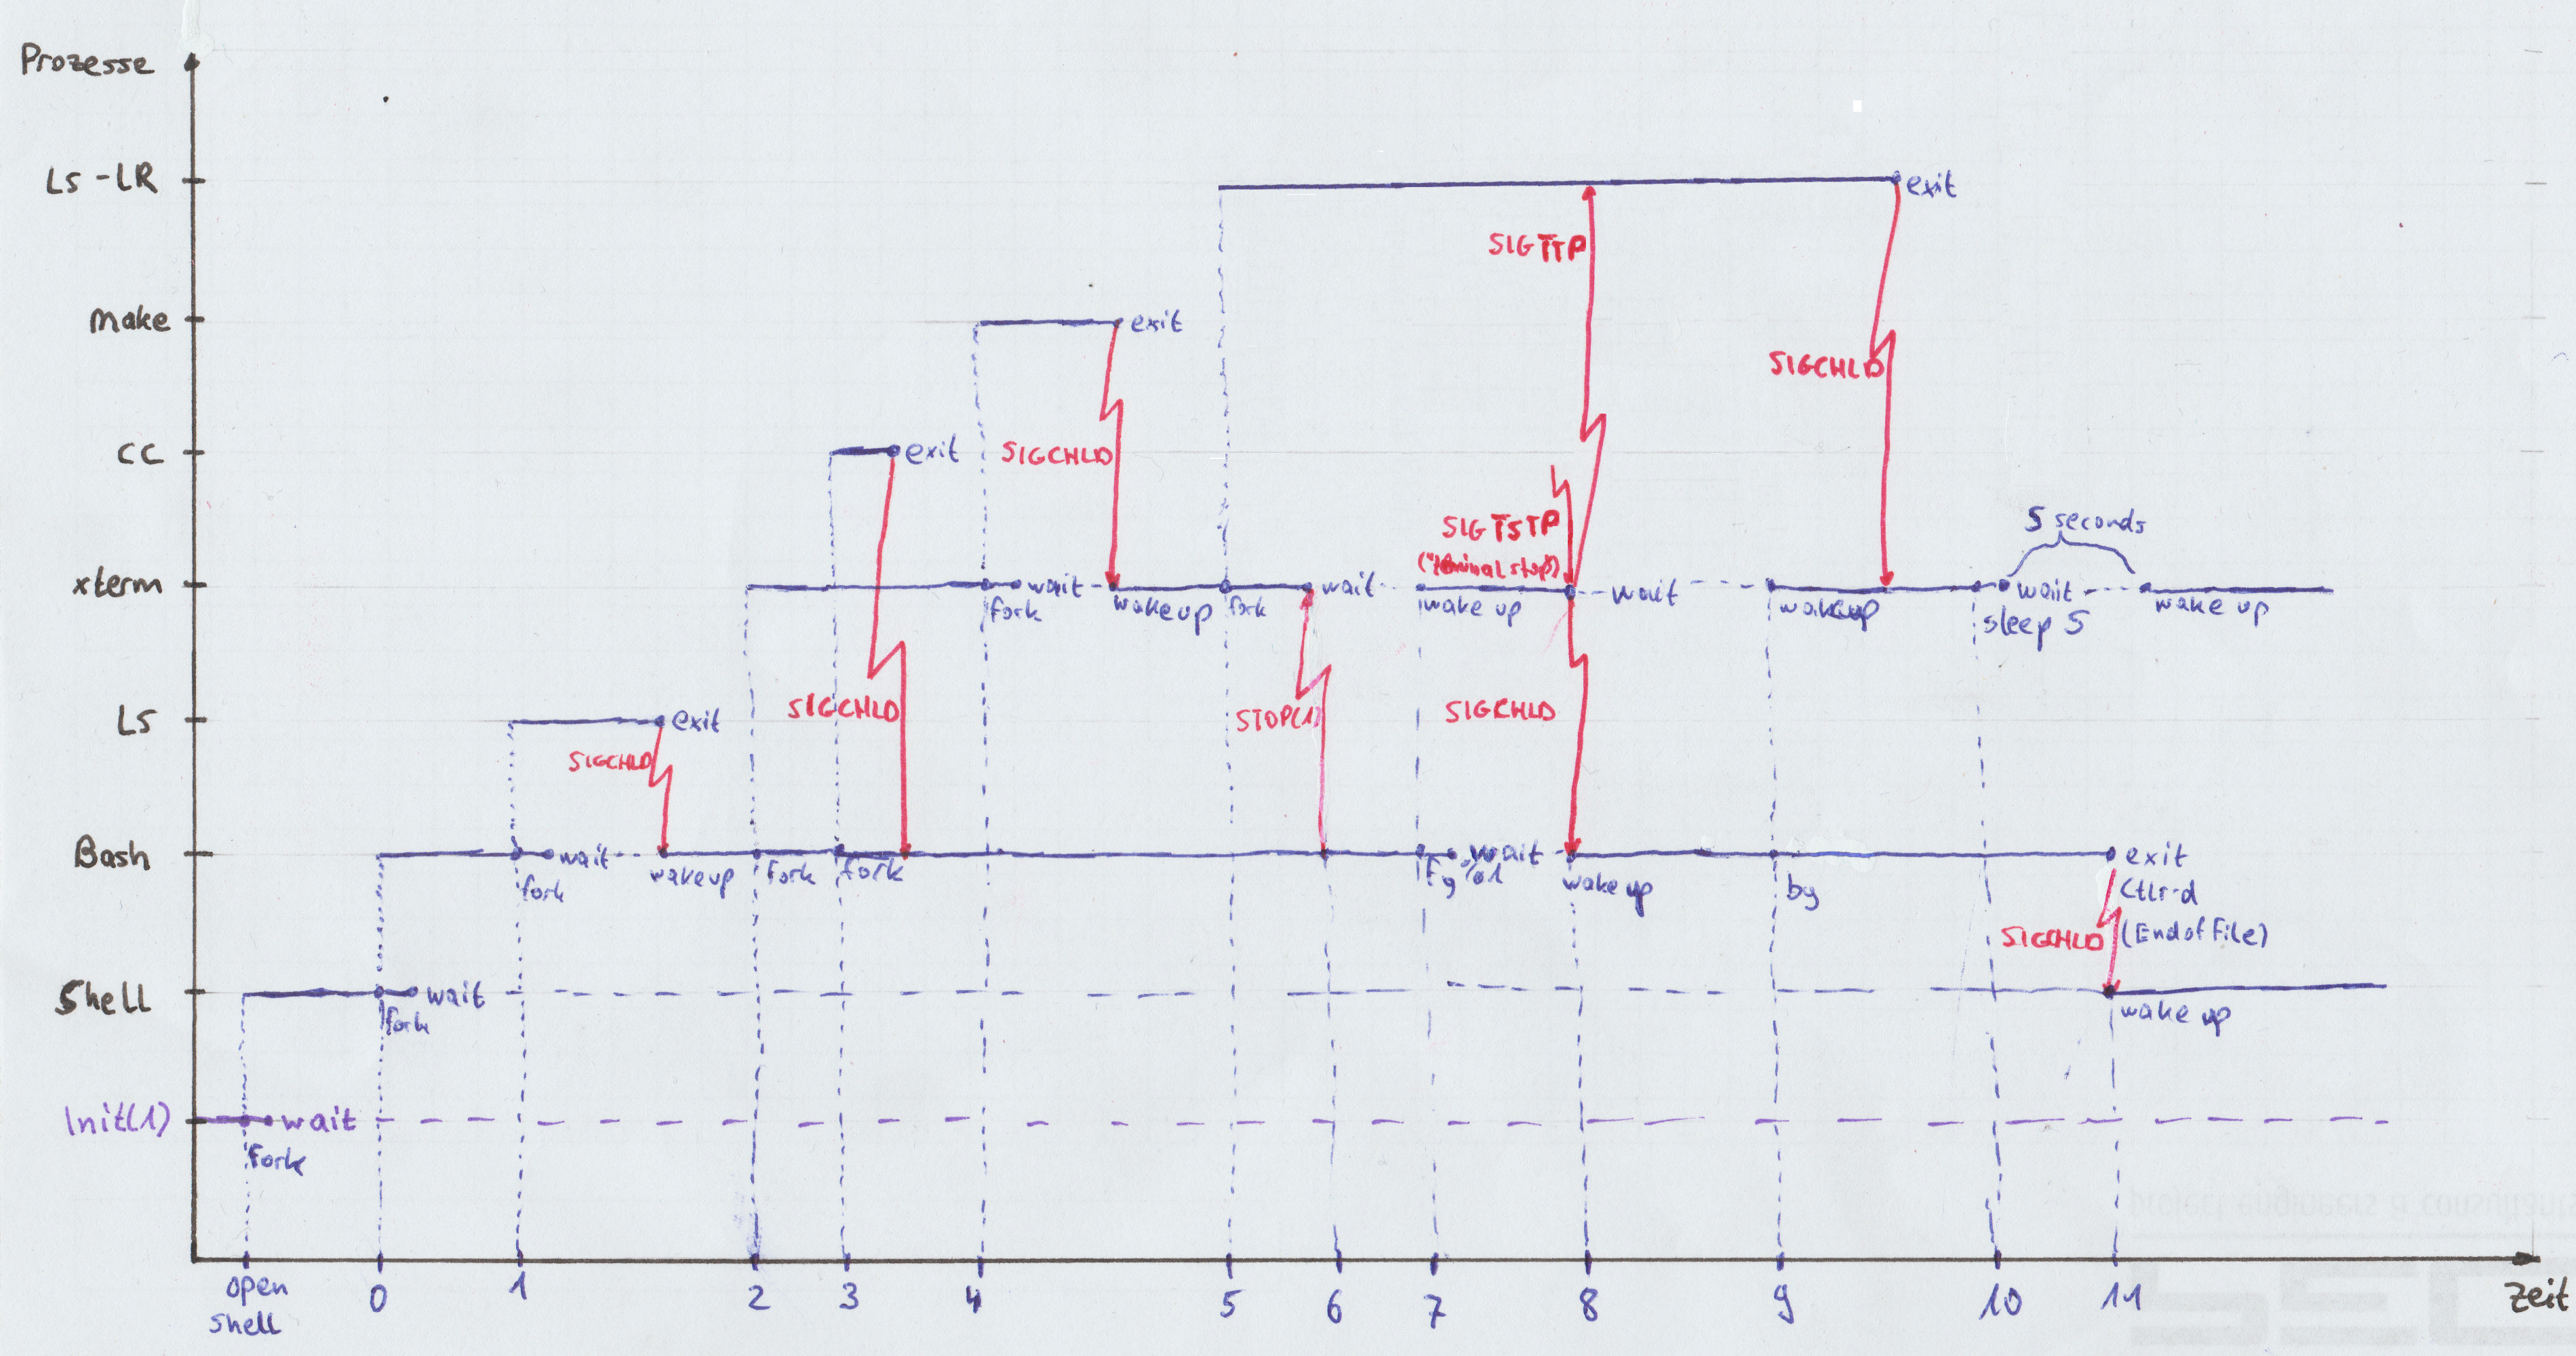
\includegraphics[width=1.1\textwidth]{Loesung/03/process-diagram.jpeg}
	\caption{Prozessdiagramm}
	\label{fig1}
\end{figure}
\textbf{Erläuterung der Befehle bzw. Prozesse}\\ \\
\begin{enumerate}
	\item \texttt{\textbf{bash}}: startet einen \textbf{bash}-Prozess innerhalb der \textbf{Shell}. Danach läuft ein \textbf{bash}-Prozess in dem \textbf{Shell}-Fenster über dem \textbf{Shell}-Prozess.
	\item \texttt{\textbf{ls}}: Zeigt den Inhalt d.h. Ordner und Verzeichnisse des aktuellen Verzeichnisses an.
	\item \texttt{\textbf{xterm \&}}: Öffnet neue \textbf{Shell} in seperatem Fenster des X-Window-Systems.
	\item \texttt{\textbf{cc baz.c \&}}: Kompiliert die Datei \textit{baz.c} zu einer \textit{a.out}-Datei.
	\item \texttt{\textbf{make}}: Rekompiliert, wenn eine \textit{make}-Datei existiert.
	\item \texttt{\textbf{ls -lR / \&}}: Zeigt den Inhalt d.h. Ordner und Verzeichnisse, sowie aller Unterverzeichnisse des gesamten Systems in detaillierter Form an. Durch \& wird der Prozess im Hintergrund ausgeführt. Dabei kann die \textbf{Shell} des \textbf{xterm}-Fensters allerdings trotzdem nicht gentutzt werden, weil die Ausgabe von \texttt{ls} immer noch in der \textbf{Shell} erfolgt.
	\item \texttt{\textbf{kill -STOP 12345}}: Das Programm \texttt{kill} sendet mit der Option \texttt{STOP} ein \textbf{SIGSTOP}-Signal an den Prozess des \textbf{xterm}-Fensters (\textbf{process id:} 12345). Es wird zwar eine Kopie der Signalanordungen (\textit{Signal dispositions}) des Vaterprozesses, welche bestimmen wie sich ein Prozess verhält, wenn es ein Signal geliefert bekommt, an Kindsprozesse die mit \texttt{fork} erstellt wurden vererbt, allerdings wird das Signal \textbf{SIGSTOP} nicht von Kindsprozessen behandelt. Deshalb wird das \textbf{SIGSTOP}-Signal, welches als Kopie gesendet wird nicht von dem Prozess \texttt{\textbf{ls -lR / \&}} behandelt. Allerdings wird die Ausgabe d.h. der \texttt{write}-Systemaufruf gestoppt. Dieser wird erst fortgesetzt, wenn der \textbf{xterm}-Prozess fortsetzt.
	\item \texttt{\textbf{fg \%1}}: Startet den ersten Prozess (bzw. \textbf{job}) der \textbf{Shell-Job}-Tabelle im Vordergrund. Dies ist in diesem Fall der \textbf{xterm}-Prozess.
	\item \texttt{\textbf{Ctrl-z}}: sendet ein \textbf{SIGTSTP}-Signal (\textit{terminal stop}) an den \textbf{xterm}-Prozess der zu Zeitpunkt des Aufrufs im Vordergrund läuft. Auch hiervon wird der \textbf{ls -lR / \&}-Prozess nicht beeinträchtigt.
	\item \texttt{\textbf{bg}}: Der \textbf{xterm}-Prozess wird im Hintergrund fortgesetzt.
	\item \texttt{\textbf{sleep 5}}: Der \textbf{xterm}-Prozess pausiert für 5 Sekunden.
	\item \texttt{\textbf{Ctrl-d}}: Ist die Eingabe der Shell bzw. hier des \textbf{Bash}-Prozesses leer löst die Tastenkombination eine \textit{End-Of-File}-Bedingung aus. Die Tastenkombination ist auch der Standardwert für das \textit{End-Of-File}-Spezialkontrollzeichen (\texttt{\textbackslash 04}). Der Terminaltreiber leitet beim drücken der Tastenkombination die gesamte Zeile der aktuellen Eingabe weiter, sodass \texttt{read()} ausgeführt wird. Ist die aktuelle Zeile leer gibt \texttt{read()} 0 zurück. Dies signifiziert der Applikation in diesem Fall dem \textbf{Bash}-Prozess, dass die \textit{End-Of-File}-Bedingung zutrifft und keine Daten mehr gelesen werden können. Der \textbf{Bash}-Prozess beendet sich selbst. 
\end{enumerate}
\begin{quote}
Wann entstehen neue Prozesse, wann terminieren sie wieder?
\end{quote}
Neue Prozesse entstehen in der Aufgabe bei den Shell-Kommandos 0 bis 5. Alle weiteren Kommandos und Tastenkombinationen erzeugen keine neuen Prozesse.\\ \\
Die Prozesse der Befehle \texttt{ls}, \texttt{cc}, \texttt{make} und \texttt{ls -lR / \&} terminieren automatisch nach beendetem Programmablauf. Der \textbf{Bash}-Prozess wird durch das Zutreffen einer \textit{End-Of-File}-Bedingung beendet.
\begin{quote}
Wann wird welchem Prozess welches Signal gesendet (und von wem)?
\end{quote}
Das erste Signal wird in dem Shell-Kommando 6 gesendet. \texttt{\textbf{kill -STOP 12345}} sendet ein \textbf{SIGSTOP}-Signal an den \textbf{xterm}-Prozess. Ein \textbf{SIGTSTP}-Signal wird durch drücken der Tastenkombination \texttt{\textbf{Ctrl-z}} gesendet.
\begin{quote}
Zu welchem Prozess gehört am Ende das in Schritt 2 gestartete Terminal?
\end{quote}
Bei Termination eine Vaterprozesses wird der Kindsprozess an den \textbf{Init(1)}-Prozess vererbt. In diesem Fall terminiert der Vaterprozess \textbf{Bash} vor dem Kindsprozess \textbf{xterm}. \textbf{xterm} wird an \textbf{Init(1)} vererbt.
\end{document}
